\documentclass[10pt, a4paper, italian]{article}
\usepackage[T1]{fontenc}
\usepackage[utf8]{inputenc}
\usepackage{amsmath, amssymb, amsthm, thmtools, amsfonts, mathtools}
\usepackage{nicefrac}
\usepackage{calc}
\usepackage[pdftex, hyperindex, plainpages=false]{hyperref}
\usepackage[nameinlink]{cleveref} %load before classicthesis (clash)
%\usepackage[nochapters,pdfspacing]{classicthesis}
\usepackage{siunitx}
\usepackage[siunitx]{circuitikz}

\usepackage[a4paper]{geometry}
\usepackage{float}
\usepackage{mdframed}
\usepackage{titling}
\usepackage{booktabs}
\usepackage{graphicx}
\usepackage{caption, subcaption}
\usepackage{xcolor}
\usepackage[italian]{babel}
\usepackage{pgfplots}
\usepackage{listings}
%\usepackage{lmodern}
\usepackage{url}
\usepackage{enumitem}
\usepackage{tikz} %loads after classicthesis (xcolor incompat)

% lets graphicx know path where figures to be included are found
\graphicspath{{../figs/}}
\makeatletter
\def\input@path{{../figs/}}
%or: \def\input@path{{/path/to/folder/}{/path/to/other/folder/}}
\makeatother

% tikz pgf plots setup
\usepgfplotslibrary{external}
\pgfplotsset{compat=1.15}
%\tikzexternalize

% spaces and significant digits/figures for measurements
\sisetup{free-standing-units, space-before-unit, number-unit-product = \;,
scientific-notation = false, round-mode = figures, round-precision = 1,}

% turns all (hyperlinked) references black [default is blue]
\hypersetup{
	linktoc=all,
	colorlinks=true,
	linkcolor=black
}

% code listings config
%\lstset{
%language=Python,
%basicstyle=\ttfamily,
%columns=fullflexible,
%keepspaces=true,
%}

% mdframed (for boxed text) configuration
\mdfsetup{linewidth=0.6pt}

% Default fixed font does not support bold face
\DeclareFixedFont{\ttb}{T1}{txtt}{bx}{n}{12} % for bold
\DeclareFixedFont{\ttm}{T1}{txtt}{m}{n}{12}  % for normal

% Custom colors
\usepackage{color}
\definecolor{deepblue}{rgb}{0,0,0.5}
\definecolor{deepred}{rgb}{0.6,0,0}
\definecolor{deepgreen}{rgb}{0,0.5,0}

% Commands 
\newcommand{\executeiffilenewer}[3]{%
	\ifnum\pdfstrcmp{\pdffilemoddate{#1}}%
		{\pdffilemoddate{#2}}>0%
	{\immediate\write18{#3}}\fi%
}
% input .svg --> .pdf_tex graphs
%\newcommand{\includesvg}[1]{%
%	\executeiffilenewer{#1.svg}{#1.pdf}%
%	{inkscape -z -D --file=#1.svg %
%	--export-pdf=#1.pdf --export-latex}%
%	\input{#1.pdf_tex}%
%}
% Thanks UniPi's Department of Physics E. Fermi
\newcommand{\thanksdf}{(\thanks{Dipartimento di Fisica E.~Fermi,%
Universit\`a di Pisa - Pisa, Italy.}\;)}

% hyperlink to email address
\newcommand{\mail}[1]{\href{mailto:#1}{\textsf{#1}}}

% \vec for bold vectors, instead of overarrows (now "\arrvec")
\let\arrvec=\vec
\renewcommand{\vec}[1]{\boldsymbol #1}
% replaces straight phi with slanted phi
\renewcommand{\phi}{\varphi}
% replaces straight eps with curved epsilon
\newcommand{\eps}{\varepsilon}
% abbreviation for (sub_/super^)scripts of \lim, \sum,... in inline math
\newcommand{\ds}{\displaystyle}

% blackboard/number set letters
\newcommand{\CC}{\mathbb C}
\newcommand{\HH}{\mathbb H}
\newcommand{\KK}{\mathbb K}
\newcommand{\NN}{\mathbb N}
\newcommand{\PP}{\mathbb P}
\newcommand{\QQ}{\mathbb Q}
\newcommand{\RR}{\mathbb R}
\newcommand{\ZZ}{\mathbb Z}

\newcommand{\Abs}[1]{{\left\Vert #1\right\Vert}}
\newcommand{\enclose}[1]{{\left( #1 \right)}}
\newcommand{\Enclose}[1]{{\left[ #1 \right]}}
\newcommand{\floor}[1]{\left\lfloor #1 \right\rfloor}
\newcommand{\ceil}[1]{\left\lceil #1 \right\rceil}
\newcommand{\To}{\rightrightarrows}

% Math operators
\DeclareMathOperator{\divergence}{div}
\renewcommand{\div}{\divergence}
\DeclareMathOperator{\Imaginarypart}{Im}
\renewcommand{\Im}{\Imaginarypart}
\DeclareMathOperator{\Realpart}{Re}
\renewcommand{\Re}{\Realpart}
%\DeclareMathOperator{\arg}{arg}
\DeclareMathOperator{\tg}{tg}
\DeclareMathOperator{\arctg}{arctg}
\DeclareMathOperator{\settsinh}{settsinh}
\DeclareMathOperator{\settcosh}{settcosh}
\DeclareMathOperator{\tr}{tr}
\DeclareMathOperator{\im}{im}
\DeclareMathOperator{\sgn}{sgn}
\DeclareMathOperator{\diag}{diag}

\DeclarePairedDelimiter{\norm}{\lVert}{\rVert}
\DeclarePairedDelimiter{\scalar}{\langle}{\rangle}

% Logarithm with arbitrary base.
% -> log_10
\newcommand{\llog}[1][10]{\log_{#1}}

% Absolute value.
% -> |x|
\newcommand{\abs}[1]{\left| #1 \right|}

% Powers.
% -> x^a
\newcommand{\power}[2][2]{\left( #2 \right)^{#1}}

% Square.
% -> x^2
\newcommand{\sq}[1]{\power[2]{#1}}

% Expansion of the binomial coefficient.
% -> n1!/(n2!(n1 - n2)!)
\newcommand{\binomexpr}[2]{\frac{#1!}{#2!(#1 - #2)!}}

% Expression evaluation at a given point with square brackets.
% -> [x]_{a}
\newcommand{\at}[2]{\left[ #1\right]_{\makebox[-1pt][l]{${\scriptstyle#2}$}}}

% Expression evaluation in an interval.
% -> [x] _{a}^{b}
\newcommand{\eval}[3]{\left.#1%
  \right|_{\makebox[-1pt][l]{${\scriptstyle#2}$}}^{\makebox[-1pt][l]{${\scriptstyle#3}$}}}

% Upright d in math mode (for differentials).
% -> d
\newcommand{\ud}{\mathrm{d}}

% Differential.
% -> dx
\newcommand{\diff}[1][x]{\,\ud{#1}}

% Base command for defining derivatives.
% -> df/dx or d^kf/dx^k
\newcommand{\basederivative}[4][]{%
  \displaystyle%
  \ifx\\#1\\\frac{#4#2}{#4#3}%
  \else%
  \frac{#4^#1#2}{#4#3^#1}%
  \fi%
}

% Total derivative.
% -> df/dx(x) or d^kf/dx^k(x)
\newcommand{\td}[4][]{%
  \basederivative[#1]{#2}{#3}{\ud}%
  \ifx\\#4\\%
  \else%
  \mkern-4mu\left(#4\right)%
  \fi%
}

% Partial derivative.
% -> df/dx(x) or d^kf/dx^k(x)
\newcommand{\pd}[4][]{%
  \basederivative[#1]{#2}{#3}{\partial}%
  \ifx\\#4\\%
  \else%
  \mkern-4mu\left(#4\right)%
  \fi%
}

\newcommand{\intinf}{\int_{-\infty}^{\infty}\!\!\!}

\newcommand{\cinterval}[2]{\left[\, #1,~#2 \,\right]}

\newcommand{\linterval}[2]{\left[\, #1,~#2 \,\right)}

\newcommand{\rinterval}[2]{\left(\, #1,~#2 \,\right]}

\newcommand{\ointerval}[2]{\left(\, #1,~#2 \,\right)}

\newcommand{\prob}[1]{\displaystyle P\left(#1\right)}

\newcommand{\pvalue}{\emph{$p$-value}}

\newcommand{\cond}{\,|\,}

\newcommand{\expect}[1]{\displaystyle E\left[#1\right]}

\newcommand{\mom}[2][]{\displaystyle {\cal M}_{#2}\ifx\\#1\\\else(#1)\fi}

\newcommand{\momalg}[1]{\displaystyle \lambda_{#1}}

\newcommand{\momcen}[1]{\displaystyle \mu_{#1}}

\newcommand{\skewness}{\displaystyle \gamma_1}

\newcommand{\kurtosis}{\displaystyle \gamma_2}

\newcommand{\charf}[1][x]{\phi_{#1}}

\newcommand{\momgenf}[1][x]{M_{#1}}

\newcommand{\fwhm}{{\scriptstyle \textsc{FWHM}}}

\newcommand{\hwhm}{{\scriptstyle \textsc{HWHM}}}

\newcommand{\median}{\mu_{\nicefrac{1}{2}}}

\newcommand{\var}[1]{\ensuremath{\text{Var}\left(#1\right)}}

\newcommand{\cov}[2]{\ensuremath{\text{Cov}\left(#1, #2\right)}}

\newcommand{\corr}[2]{\ensuremath{\text{Corr}\left(#1, #2\right)}}

\newcommand{\like}{\mathcal L}

\newcommand{\likelihood}[2][]{\like\ifx\\#2\\\else(#2\ifx\\#1\\\else;#1\fi)\fi}

\newcommand{\chisq}{\ensuremath{\chi^2}}

\newcommand{\chisquare}[2][]{\chisq\ifx\\#2\\\else(#2\ifx\\#1\\\else;#1\fi)\fi}

\newcommand{\loglikelihood}[2][]{\log\likelihood[#1]{#2}}

\newcommand{\pdf}[3][]{#2(#3\ifx\\#1\\\else;#1\fi)}

\newcommand{\binomialpdf}[2][]{\pdf[#1]{\mathcal B}{#2}}

\newcommand{\multinomialpdf}[2][]{\pdf[#1]{\mathcal M}{#2}}

\newcommand{\poissonpdf}[2][]{\pdf[#1]{\mathcal P}{#2}}

\newcommand{\uniformpdf}[2][]{\pdf[#1]{u}{#2}}

\newcommand{\exponentialpdf}[2][]{\pdf[#1]{\varepsilon}{#2}}

\newcommand{\gausspdf}[2][]{\pdf[#1]{N}{#2}}

\newcommand{\chisquarepdf}[2][]{\pdf[#1]{\wp}{#2}}

\newcommand{\cauchypdf}[2][]{\pdf[#1]{c}{#2}}

\newcommand{\erf}[1]{\ensuremath{\text{erf}\left(#1\right)}}

\newcommand{\dccases}[4][]{#2 \ifx\\#2\\\else=\fi %
  \begin{cases}
    \displaystyle #3 & \text{per variabili discrete}\\
    \displaystyle #4 & \text{per variabili continue}#1
  \end{cases}
}
% sub/super-scriptable for all symbol as math operator 
\newcommand\Scaleforall[1]{\vcenter{\hbox{\scalefont{#1}$\forall$}}}

\DeclareMathOperator*\forevery{%
  \vphantom\sum
  \mathchoice{\Scaleforall{2}}{\Scaleforall{1.4}}{\Scaleforall{1}}{\Scaleforall{0.75}}}
\geometry{left=2cm, right=2cm, top=2cm, bottom=2cm}

% indexes subsections with letters, sections with numbers (1.a, 1.b, ...)
\renewcommand{\thesubsection}{\thesection.\alph{subsection}}

% lets graphicx know path where figures to be included are found
\graphicspath{{../figs/}}

\author{Gruppo 1.AC \\ Matteo Rossi, Bernardo Tomelleri}
\title{Es09: Misura della velocità del suono}
\begin{document}
\date{\today}
\maketitle

\setcounter{section}{0}

\section*{Misura componenti dei circuiti}
\begin{table}[htbp]
\centering
\begin{tabular}{ccc|ccc}
\toprule
Resistenze $[\si{k\ohm}]$ & $R$ & $\sigma R$ & Resistenze $[\si{k\ohm}]$ & $R$ &
$\sigma R$ \\
\midrule
\midrule
$R_1$	  	& 9.95 	& 0.08		& $R_1$ & 9.98	& 0.08 \\
\bottomrule
\end{tabular}
\caption{Valori di resistenza misurate con il multimetro dei componenti dei
due circuiti studiati. \label{tab: rcmes_B}}
\end{table}

Riportiamo per completezza anche il valore della tensione di alimentazione
continua per il sensore a ultrasuoni misurata con il multimetro.
\[
V_{CC} = 4.99 \pm 0.03 \si{\V}
\]

\subsection*{Nota sul metodo di fit}
Per determinare i parametri ottimali e le rispettive covarianze si \`e
implementato in \verb+Python+ un algoritmo di fit basato sui minimi quadrati
mediante la funzione \emph{curve\_fit} della libreria \texttt{SciPy}.

%=======================
\section{Misura velocità del suono}
\subsection{Progettazione del circuito}
Si è costruito il nostro apparato per la misura della velocità del suono
secondo lo schema circuitale riportato in \cref{schm: mesctrl}.
\begin{figure}[htbp]
    \centering
	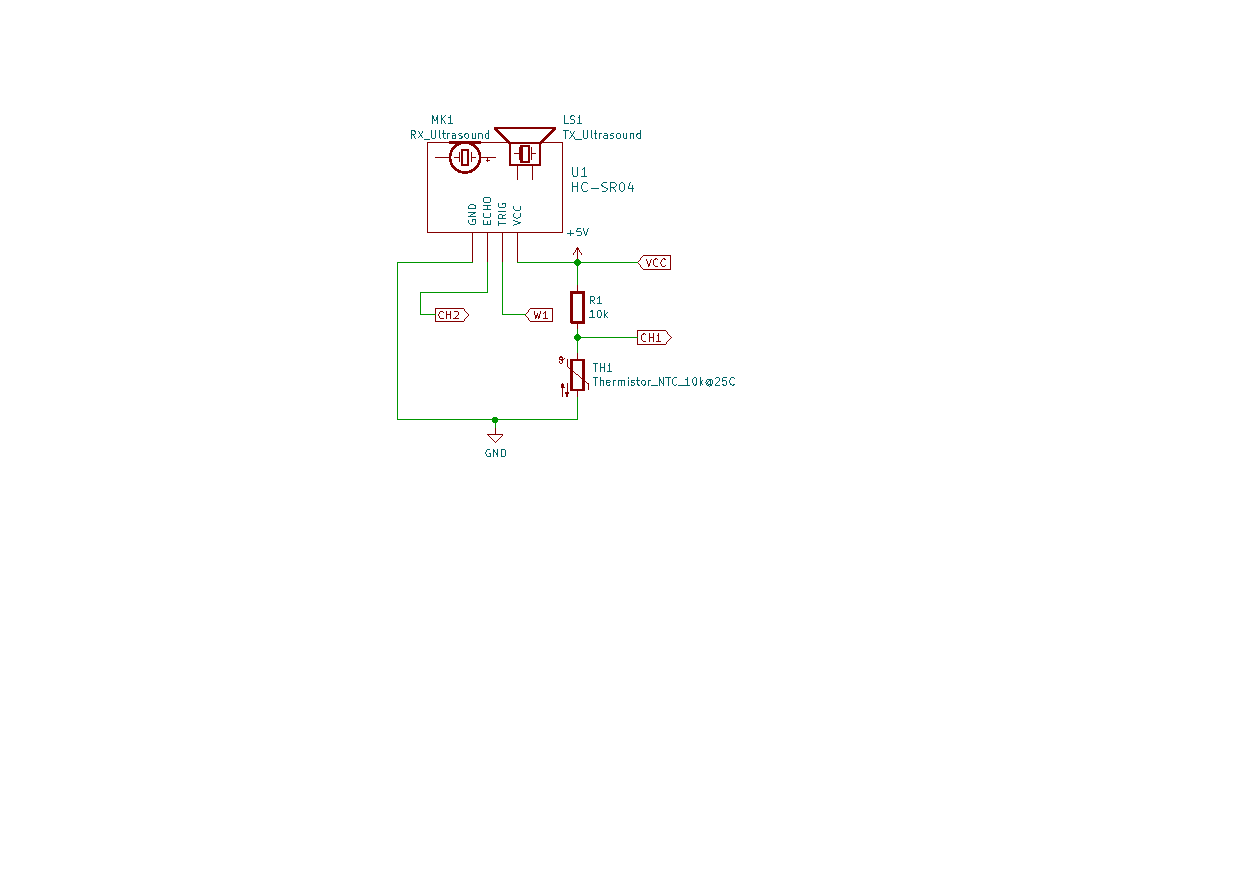
\includegraphics[scale=1]{schm}
    \caption{Schematica del circuito per la misurazione della velocità del
    suono e della temperatura. I due sotto-circuiti condividono la stessa
    tensione di alimentazione $V_{CC}$.
    \label{schm: mesctrl}}
\end{figure}

In cui si è cercato di mettere in evidenza la geometria del componente
principale, il sensore ad ultrasuoni di tipo riflettente HC-SR04, in cui
il trasmettitore ed il ricevitore sono separati di una distanza di circa
$\SI{2}{c\m}$.

Nello stesso schema si riporta anche il sotto-circuito di misura della
temperatura ambientale, costituito da un partitore di tensione/la
serie di due resistori, il secondo dei quali ha valore di resistenza $R_T$
dipendente dalla temperatura.

\subsection{Analisi del funzionamento dell'apparato}
Il sensore ad ultrasuoni fornisce una stima del tempo di viaggio $t$ in aria
(andata e ritorno) di un'onda sonora dalla frequenza superiore alla soglia
dell'udito umano $\sim 20 \; \si{k\Hz}$ sotto forma di un impulso TTL di
durata proporzionale a $t$.

Sempre per la convenzione TTL il sensore dev'essere alimentato da una
differenza di potenziale di livello alto $+\SI{5}{\V}$ e per avviare il
processo di misura al pin \verb+TRIG+ si deve inviare un segnale di trigger
(un impulso che deve soddisfare le condizioni di ampiezza, durata e periodo
specificate nel datasheet del componente). Nel nostro caso si è generata in
\verb+W1+ una serie di impulsi compresi tra 0 e $\SI{5}{\V}$ di durata pari a
$10 \si{\micro\s}$ e periodo di $50 \; \si{m\s}$, per permettere all'HC-SR04
di portare a termine il suo ciclo di misura (scelto in base alla durata
massima del segnale di eco $\sim 38 \; \si{m\s}$, corrispondente al caso in
cui il ricevitore non rileva alcun ostacolo che riflette gli impulsi emessi)
e torni ad essere pronto a ricevere un nuovo impulso di trigger da $W_2 (t)$.

Sul fronte di discesa dell'impulso di trigger il sensore genera un segnale
continuo alto nel pin \verb+ECHO+ e un'onda sonora costituita da un treno
d'impulsi da $f = 40 \; \si{k\Hz}$ nel trasmettitore.
Questa si propaga finché non incontra un ostacolo piano e opaco da cui viene
riflesso in modo da essere captato dal ricevitore piezoelettrico nel sensore
al ritorno. Non appena il cristallo piezoelettrico riceve uno di questi
impulsi di ritorno emessi ogni $1/f = 25 \; \si{m\s}$ il segnale alto presente
nel pin \verb+ECHO+ torna ad essere $SI{0}{\V}$. Controllando quindi
quest'ultimo pin tramite l'oscilloscopio è possibile osservare un gradino di
tensione dalla durata direttamente proporzionale al tempo $t$ che l'onda a
ultrasuoni impiega a percorrere 2 volte la distanza $D$ tra il sensore e
l'oggetto riflettente.
\begin{figure}[htbp]
    \centering
	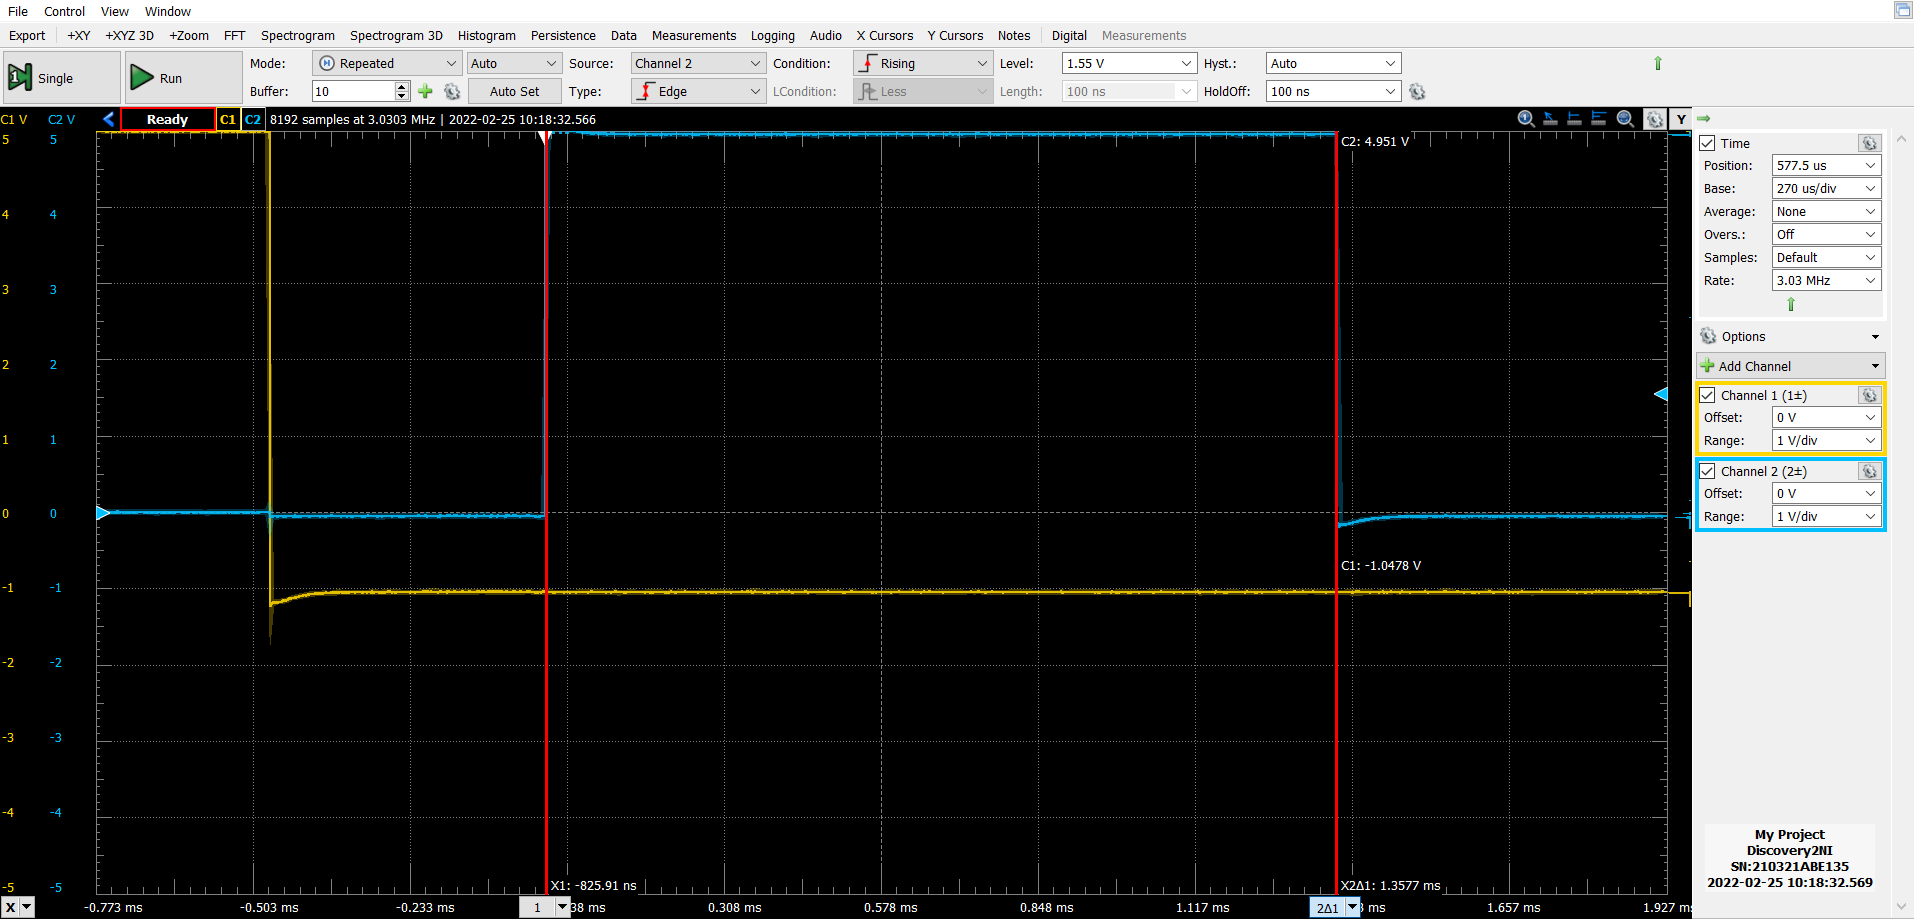
\includegraphics[scale=0.4]{echo}
    \caption{Acquisizione all'oscilloscopio dei segnali di trigger $W_2 (t)$
    (in giallo, su CH1) e $V\ped{ECHO} (t)$ (in blu, su CH2) per una misura
    con bersaglio a una distanza $D = \SI{15}{cm}$.}
\end{figure}

In contemporanea al ciclo di misura dell'HC-SR04 si monitora la temperatura
dell'aria circostante misurando l'uscita del partitore di tensione/la caduta
di tensione ai capi del termistore $V_T$ con $R_0 = 10 \pm 1 \percent \;
\si{k\ohm}$ (tabulata da datasheet a temperatura ambiente $\sim 25 \;
\degreeCelsius$).

\subsection{Raccolta e analisi dati}\label{sbs: data}
Dunque una volta misurata la distanza sensore-oggetto con un metro a nastro,
è possibile ricavare la velocità del suono dalle misure di tempo fornite dal
sensore tramite la \cref{eq: d/t}
\begin{equation}\label{eq: d/t}
v = \frac{2 D}{t}
\end{equation}

Avendo cura di incidere su un oggetto quanto meno scabro, fisso e a distanza
$D$ abbastanza grande da poter trascurare la distanza $b \approx 2 \; \si{cm}$
tra trasmettitore e ricevitore dell'HC-SR04 nel tragitto del segnale a
ultrasuoni; si è proceduto con la misura dei tempi di viaggio al variare di
$D$ facendo avanzare l'apparato lungo delle guide rettilinee. In particolare
si è scelto di ripetere la presa dati sia per distanze brevi (tra $15$ e
$25 \; \si{c\m}$) e distanze più lunghe (dai $25$ ai $44 \; \si{c\m}$) ma
comunque sotto i $50 \; \si{c\m}$ per ridurre l'influenza di interferenza da
parte di altri corpi lungo il percorso dell'onda trasmessa.

Nel primo caso (distanze brevi) per misurare correttamente la distanza e
ridurre la sua incertezza associata, si è stimata la posizione del cristallo
piezoelettrico nei canali del trasmettitore e del ricevitore inserendo una
piccola sonda all'interno dei due occhi del sensore. Da cui abbiamo ricavato
che ci sono circa $h = 5 \pm 1 \; \si{m\m}$ di distanza tra il cristallo e la
rete di protezione esterna, quindi si è scelto di prendere come incertezza
sulla distanza percorsa $\SI{2}{m\m}$. Nell'altro esperimento si è invece
misurata la distanza $D$ a partire dal punto di mezzo dei canali di lunghezza
$a = 15 \; \si{m\m}$ (dal datasheet), per cui si è associata un incertezza
$\sigma D = a/2$.

Per quanto riguarda le misure di $t$ invece abbiamo sempre utilizzato i
cursori sulla scala dei tempi dell'oscilloscopio per monitorare la durata
dell'impulso in \verb+ECHO+. Tutto questo controllando che la temperatura
rimanesse costante durante le prese dati, sia grossolanamente con le
termocoppie del multimetro, sia assicurandoci che la caduta di
tensione ai capi del termistore rimanesse costante nel tempo entro
l'incertezza.
\begin{table}[htbp]
\centering
\begin{tabular}{cc}
\toprule
Travel Time $t$ $(\pm 0.02)$ [ms] & Distance $D$ $(\pm 0.2)$ [cm] \\
\midrule
\midrule
0.86 & 15.0 \\
0.92 & 16.0 \\
0.98 & 17.0 \\
1.03 & 18.0	\\
1.10 & 19.0 \\
1.15 & 20.0 \\
1.21 & 21.0 \\
1.27 & 22.0 \\
1.32 & 23.0 \\
1.39 & 24.0 \\
\bottomrule
\end{tabular}
\caption{Distanze e tempi di viaggio misurati nell'esperimento su distanze
brevi.}
\end{table}

\begin{table}[htbp]
\centering
	\begin{tabular}{cc}
	\toprule
	Travel time $t$ $(\pm 0.02)$ [ms] & Travel length $s = 2D$ $(\pm 1.5)$ [cm] \\
	\midrule
	\midrule
	1.44                              & 50.4                                  \\
	1.50                              & 52.4                                  \\
	1.56                              & 54.0                                  \\
	1.60                              & 56.4                                  \\
	1.65                              & 58.2                                  \\
	1.71                              & 60.0                                  \\
	1.74                              & 62.2                                  \\
	1.83                              & 64.4                                  \\
	1.88                              & 66.4                                  \\
	1.94                              & 68.2                                  \\
	2.00                              & 70.0                                  \\
	2.05                              & 72.0                                  \\
	2.11                              & 74.0                                  \\
	2.18                              & 75.6                                  \\
	2.23                              & 78.4                                  \\
	2.29                              & 80.0                                  \\
	2.33                              & 82.0                                  \\
	2.41                              & 84.0                                  \\
	2.47                              & 86.0                                  \\
	2.51                              & 88.0                                  \\
	\bottomrule
	\end{tabular}
	\caption{Distanze percorse e tempi di viaggio misurati nell'esperimento su
	distanze lunghe.}
\end{table}

Infine si è eseguito un fit lineare a partire dal grafico delle distanze
percorse $s(t) = 2D = v_s t + q$ in funzione del tempo per ricavarne dal
coefficiente angolare la misura della velocità del suono $v_s$ di nostro
interesse.
\begin{figure}[htbp]
    \centering
	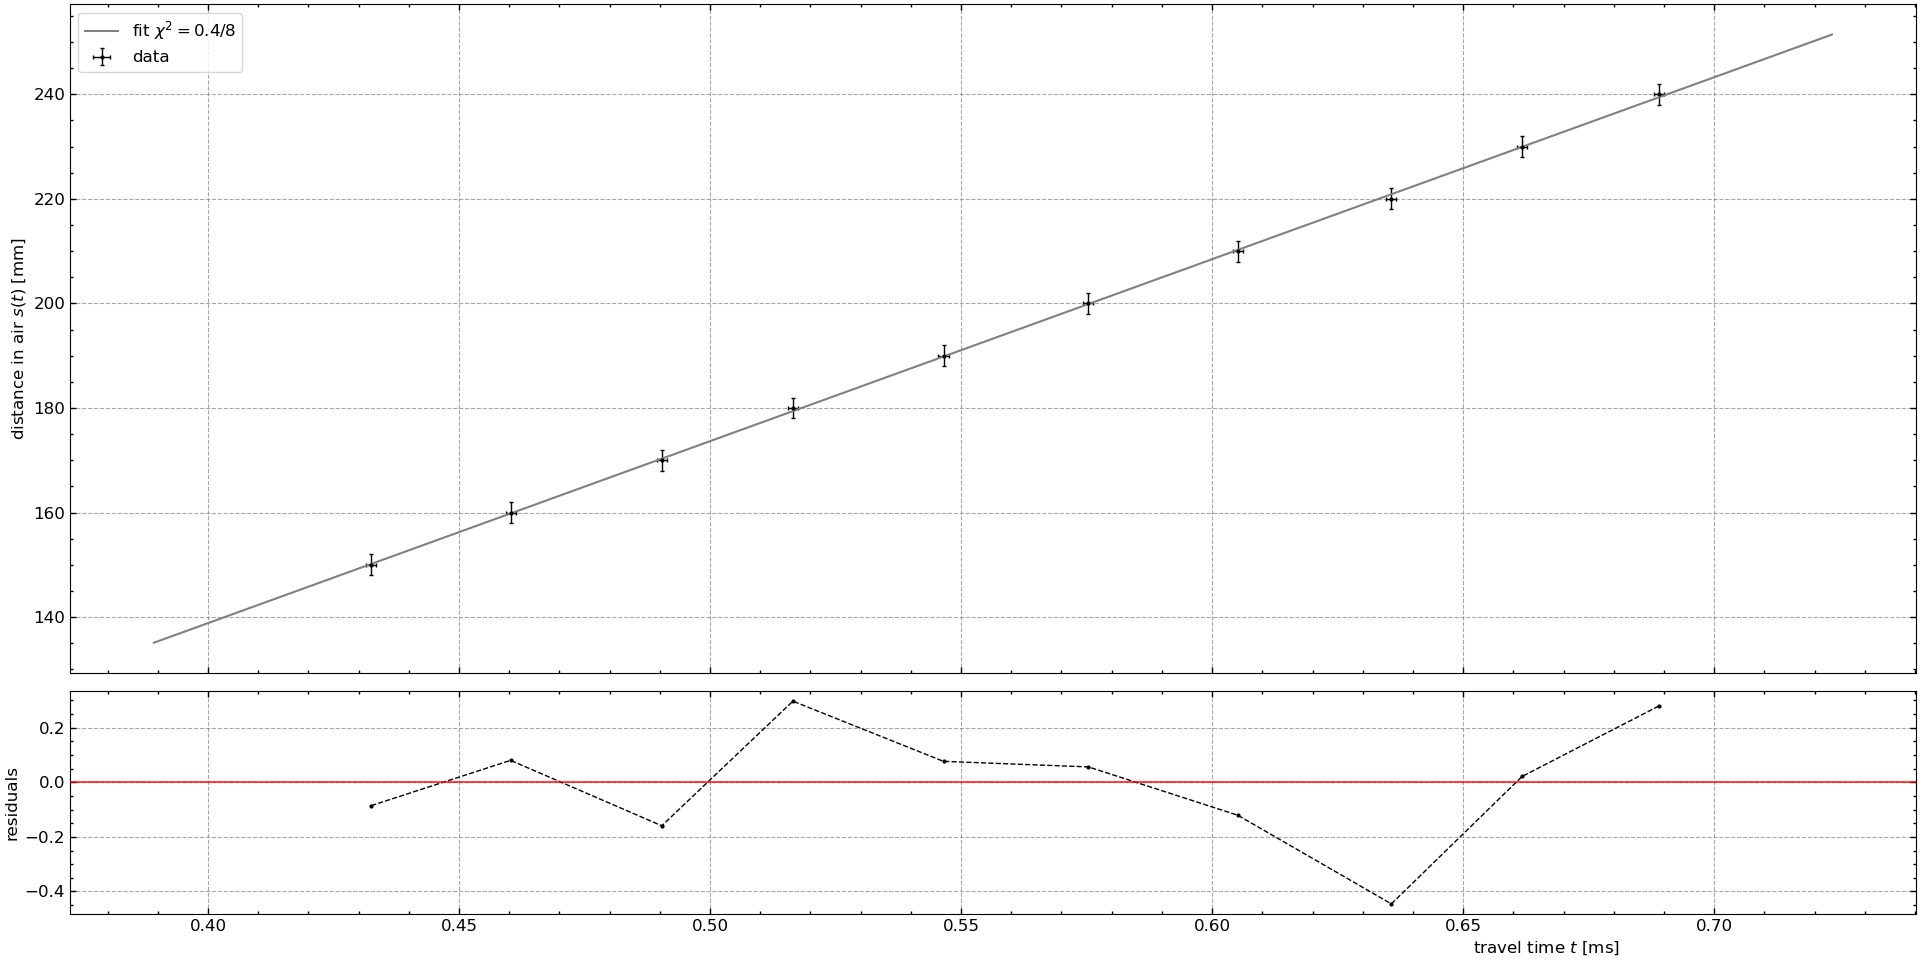
\includegraphics[width=\textwidth]{2}
    \caption{Fit lineare all'andamento delle distanze (corte) in funzione del
    tempo}
\end{figure}
\begin{figure}[htbp]
    \centering
	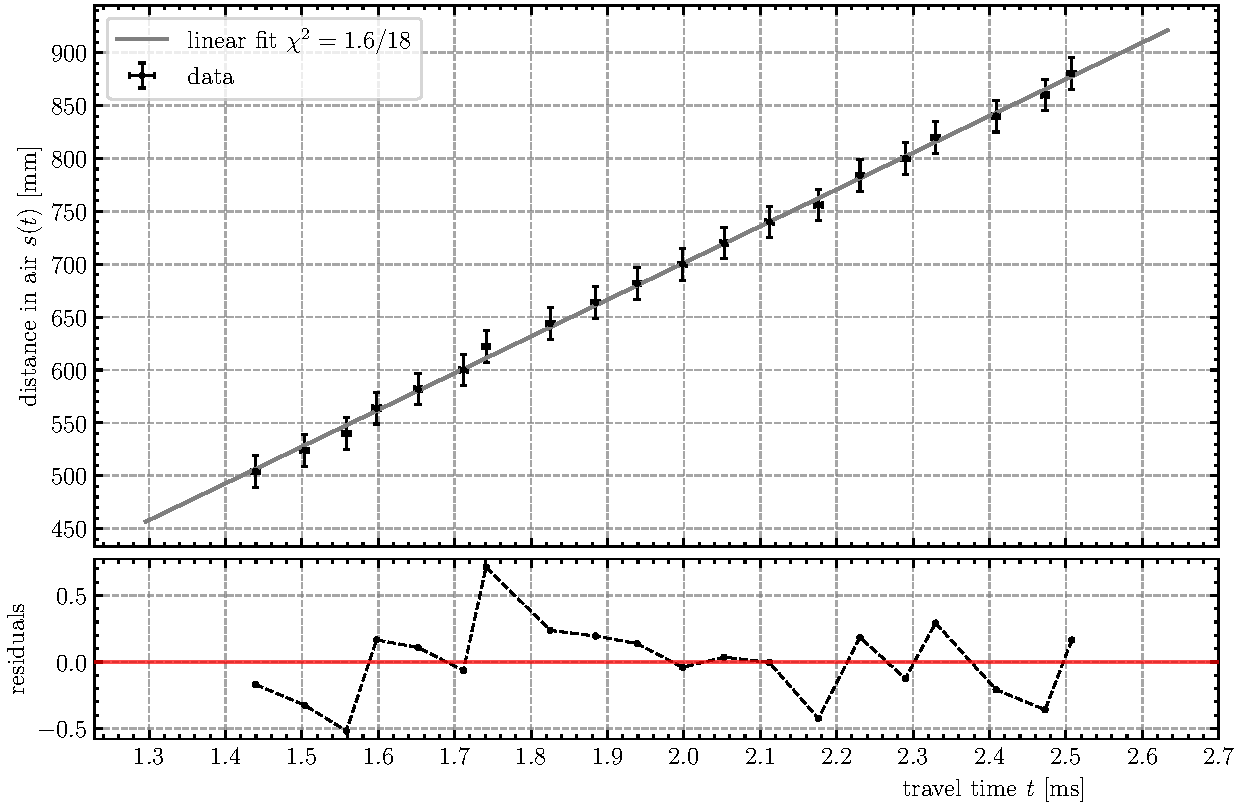
\includegraphics[width=\textwidth]{railtime}
    \caption{Fit lineare all'andamento delle distanze (lunghe) in funzione del
    tempo}
\end{figure}

\begin{table}[htbp]
\centering
\begin{tabular}{cccc|c}
\toprule
$v_s$ [m/s]& $q$ [mm] & $\chi^2/\text{d.o.f}$ & norm. cov. &
Temperature $T$ [\degreeCelsius] \\
\midrule
\midrule
$348 \pm 2$ & $0.4 \pm 1.0$ & $0.4/6$ & $-0.97$ & $20 \pm 1$ \\
$347 \pm 3$ & $0 \pm 6$ & $1.6/18$ & $-0.99$ & $21 \pm 1$ \\
\bottomrule
\end{tabular}
\caption{Risultati del fit lineare per la velocità del suono dalle misure
su distanze brevi e lunghe rispettivamente}
\end{table}

In entrambi i casi abbiamo ottenuto un'intercetta compatibile con 0, che ci
suggerisce che le distanze tra sensore e oggetto riflettente siano state
stimate in maniera corretta entro l'incertezza.

I 2 esperimenti sono stati eseguiti all'interno di case diverse in città
diverse, quindi con condizioni di umidità relative differenti. Nonostante
questo sono risultate perfettamente compatibili tra di loro e con il valore
di riferimento per la velocità del suono di $343 \; \si{\m/\s}$ a
$20 \; \si{\degreeCelsius}$ entro meno di 3 barre d'errore.

\subsection{Jitter discreto nelle misure di tempo}
Un fenomeno che ci è sembrato meritevole di particolare attenzione è la natura
delle oscillazioni delle misure di tempo prese dal fronte di discesa del
segnale in \verb+ECHO+.
Abbiamo notato che, pur mantenendo fisso l'apparato strumentale, il tempo
in cui il segnale di eco torna ad essere $\SI{0}{\V}$ dopo aver ricevuto l'onda
riflessa tende a oscillare tra almeno un paio di valori tutti grossomodo
separati di uno stesso tempo caratteristico.

Si è provato a dare una spiegazione di questo effetto di ``jitter'' discreto 
a partire dalla schematica completa dell'HC-SR04: questo è composto da 3
circuiti principali, denominati U1, U2 e U3. Il primo e l'ultimo sono impiegati
per la generazione del segnale di eco e dell'onda sonora trasmessa, mentre U2 è
dedicato a riconoscere il segnale acustico di ritorno.
Quest'ultimo è costituito (oltre a vari altri componenti) principalmente da un
filtro passa-banda e un amplificatore; per cui collegandoci al pin 10 dell'U2
è stato possibile osservare il segnale corrispondente all'arrivo treno
d'impulsi a $40 \; \si{k\Hz}$ isolato e amplificato dal circuito.
\begin{figure}[htbp]
    \centering
	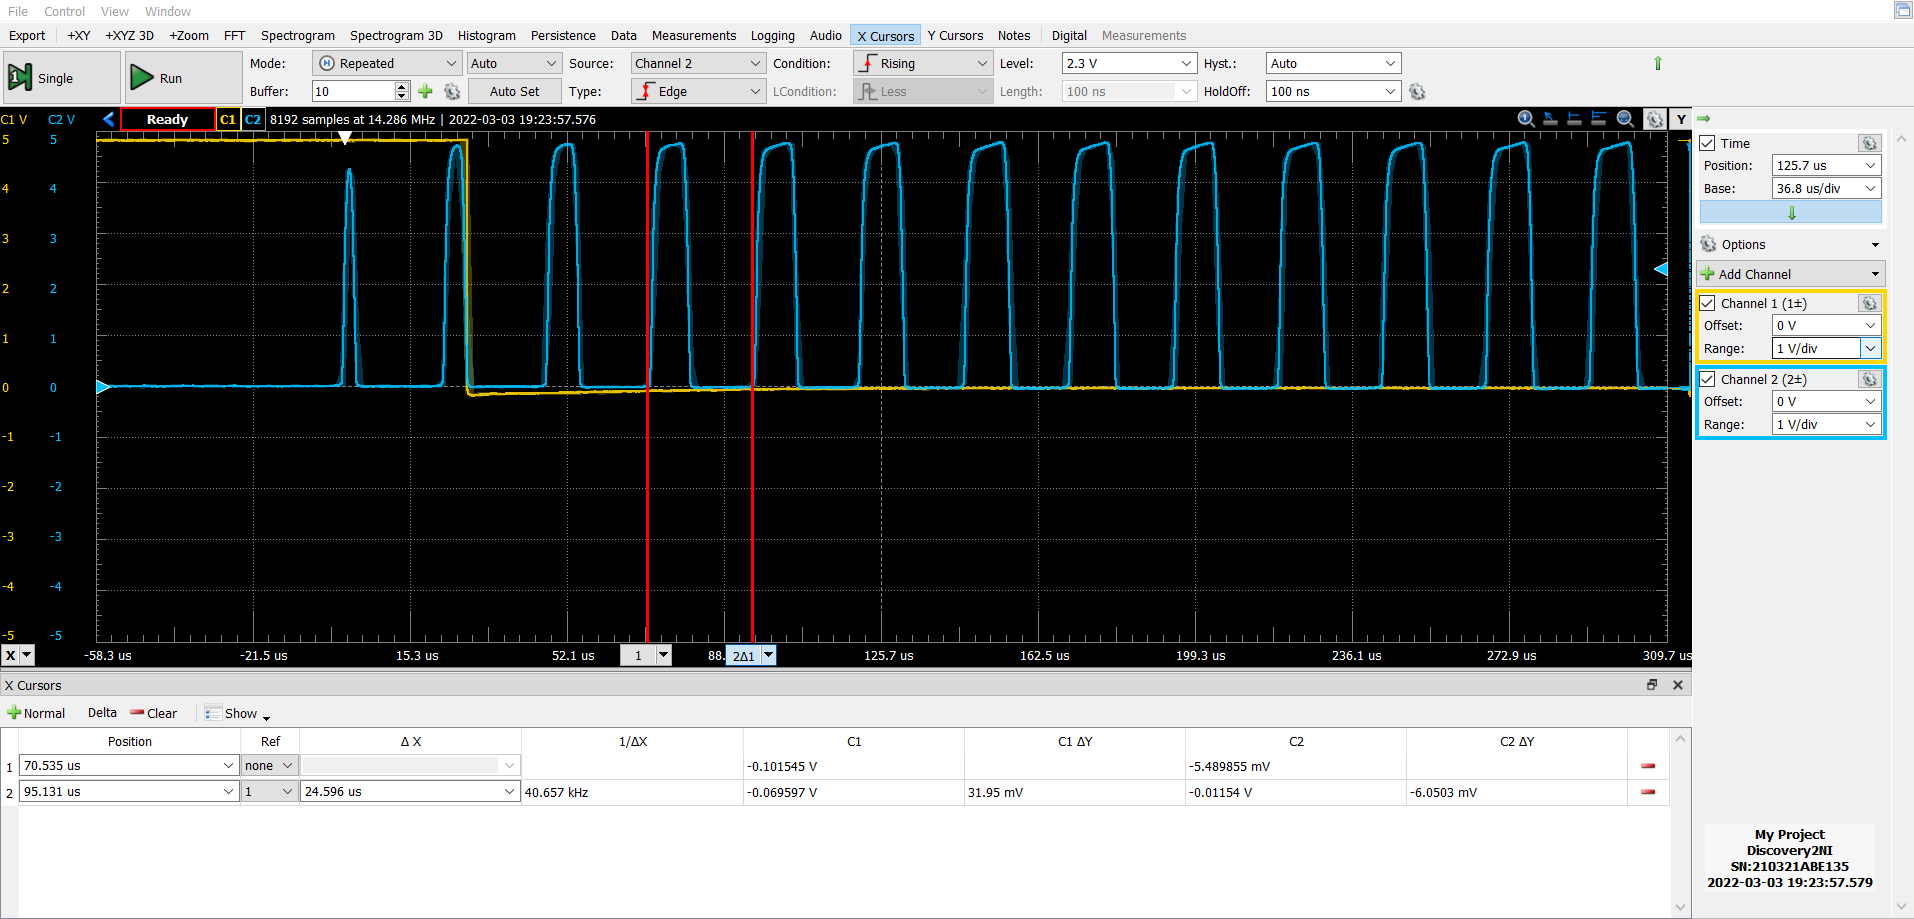
\includegraphics[width=\textwidth]{jitter2}
    \caption{Acquisizione all'oscilloscopio del segnale in uscita dal pin 10
    dell'integrato U2 (in blu su CH2) e dell'uscita in \texttt{ECHO} (in giallo
    su CH1}
\end{figure}

Da questo ipotizziamo che il jitter discreto sia dovuto al fatto che il
sensore abbassi la tensione dell'impulso in uscita da \verb+ECHO+ in maniera
inconsistente quando, ad esempio, il primo fronte dell'onda di ritorno non
genera nel trasduttore una differenza di potenziale sufficiente a farne
registrare l'arrivo dai circuiti integrati.
Misurando il ritardo tra il primo impulso e quello che fa effettivamente
scattare il segnale in \verb+ECHO+ con i cursori si trova un valore
perfettamente compatibile con $1/f = 25 \; \si{\micro\s}$, pari al
periodo dell'onda a ultrasuoni che non viene percepita dal ricevitore.

%=======================
\section{Dipendenza della velocità dalla temperatura}
Sappiamo che la velocità del suono in aria non è costante, ma varia nelle
nostre condizioni sperimentali principalmente a causa della temperatura e
dell'umidità\footnote{in linea di principio $v_s$ dipende anche dalla
frequenza dell'onda di pressione che si propaga in aria, ma stiamo
considerando un unico valore di frequenza fissato da $f = 40 \; \si{k\Hz}$}.

Non potendo monitorare né controllare le condizioni di umidità dell'aria
possiamo solamente limitarci a dire che (a parità di temperatura) ci
aspettiamo che la percentuale di umidità relativa contribuisca ad aumentare
il valore di $v_s$ misurato. Infatti, assumendo di poter esprimere la velocità
del mezzo nella forma
\begin{equation}
v_s(\rho) = \sqrt{\frac{k}{\rho}}
\end{equation}
sappiamo che la densità di massa per unità di volume $\rho$ dell'aria
diminuisce in presenza di molecole d'acqua poiché hanno massa minore di quelle
d'aria. Ad ogni modo non ci aspettiamo una deviazione dai valori attesi
(che assumono aria perfettamente secca/di umidità relativa $0 \percent$) di più
di $\sim SI{2}{\m/\s}$, quindi entro la nostra incertezza di misura.

\subsection{Descrizione del metodo di misura}
In particolare quindi ci concentriamo sulla misura della dipendenza di $v_s$
dalla temperatura tramite la misura indiretta della resistenza $R_T$ di un
termistore NTC (modello MF52D-103f-3950).

Dalla formula del partitore di tensione $R_1 + R_T$ possiamo ricavare una
stima della resistenza del termistore misurando la caduta di tensione ai suoi
capi $V_T$.
\begin{equation}
R_T = R_1 \frac{V_T}{V_{CC} - V_T} = \frac{R_1}{V_{CC}/V_T - 1}
\end{equation}

Dunque possiamo ottenere la nostra misura della temperatura assoluta $T$
(in Kelvin) dall'equazione di Steinhart-Hart
\begin{equation}\label{eq: STH}
\frac{1}{T} = \frac{1}{T_0} + \frac{\ln{\left(\frac{R_T}{R_0}\right)}}{B}
\end{equation}
da cui si vede ancora come la temperatura sia legata in maniera inversamente
proporzionale alla resistenza $R_T$.
\begin{equation}
T = \frac{T_0 B}{B + T_0 \ln{\frac{R}{R_0}}}
\end{equation}

Finalmente possiamo ottenere una stima del valore della velocità del suono a
temperatura $T_C = \SI{0}{\degreeCelsius} = 289.15 \; \si{\K} \coloneq T_0$
dall'equazione che descrive l'andamento di $v_s$ al variare di $T_C$
(espressa in gradi Celsius)
\begin{equation}\label{eq: v(T)}
v_s = v_0 \sqrt{\frac{T_C + 273.15}{273.15}}
\end{equation}

\subsection{Raccolta e analisi dati}
In questo caso abbiamo misurato il tempo $t$ di percorrenza del segnale a
ultrasuoni lasciando fissa la distanza $D = 252 \pm 2 \; \si{m\m}$
(sempre prendendo come punto di partenza delle onde $h = \SI{5}{m\m}$ dalla
fine dei canali del sensore) al variare della temperatura dell'aria nella
stanza.

Per verificare il corretto funzionamento del circuito di misura della
temperatura si è posizionato l'apparato a fianco di un termostato per eseguire
una sorta di grossolana calibrazione del termistore.
Da una misura con i cursori della caduta di tensione ai capi di $R_T$ abbiamo
ottenuto $V_T = 2.81 \pm 0.02 \si{\V}$, dunque dall'\cref{eq: STH} si ricava
una misura di temperatura $T_C = 19.4 \pm 0.4 \; \si{\degreeCelsius}$, in
ottimo accordo con la lettura indicata dal termostato di
$19.5 \; \si{\degreeCelsius}$ (il quale ha risoluzione di 1 decimo di grado).

Da cui concludiamo che i valori dei parametri di costruzione del termistore
$R_0 = 10 \; \si{k\ohm}$ e $B = 3950 \; \si{\K}$ riportati nel datasheet con
relative tolleranze dell'$1 \percent$ possono fornire una stima ragionevole
della temperatura ambientale, una volta inserite nella \cref{eq: STH}.

Nonostante basti lasciare il circuito in ciclo continuo di presa dati ed
aspettare il cambiamento naturale di temperatura nel giorno, siamo riusciti
a compiere le nostre misure entro un intervallo di soli $5 \degreeCelsius$ di
escursione termica, compresi tra i 15 e i $20 \degreeCelsius$.

In maniera del tutto analoga a prima abbiamo preso le misure dei tempi di
volo $t$ tramite cursori sulla scala dei tempi dell'oscilloscopio dalla
durata dell'impulso in \verb+ECHO+. In contemporanea si monitora la temperatura
dell'aria con le termocoppie del multimetro, il termostato e dalla lettura di
$V_T$ con i cursori sull'altro canale dell'oscilloscopio.
\begin{table}[htbp]
\centering
\begin{tabular}{cccc}
\toprule
Travel time $t$ ($\pm 0.02$) [ms] & $V_T$ $(\pm 0.02)$ [V] & $T_C$ $(\pm 0.4)$
[\degreeCelsius] & Termostato-DMM ($\pm 1$) [\degreeCelsius] \\
\midrule
\midrule
1.49 & 3.11 & 14.3 & 15 \\
1.49 & 3.03 & 15.6 & 16 \\
1.48 & 2.98 & 16.6 & 17 \\
1.48 & 2.93 & 17.5 & 18 \\
1.47 & 2.88 & 18.3 & 19 \\
1.47 & 2.83 & 19.2 & 20 \\
\bottomrule
\end{tabular}
\caption{Misure dei tempi di volo al variare della temperatura
ambientale registrata durante l'arco di una giornata.}
\end{table}

Abbiamo nuovamente usato l'\cref{eq: d/t} per ottenere le nostre misure di
velocità, dunque a partire dalle misure di temperatura ricavate da
\cref{eq: STH} si è potuto ricostruire l'andamento di $v_s$ in funzione
della temperatura $T$. Infine si è condotto un fit a questi dati con la legge
di potenza \cref{eq: v(T)} per stimare $v_0$ e verificare l'accordo con
l'andamento da questa previsto.
\begin{figure}[htbp]
    \centering
	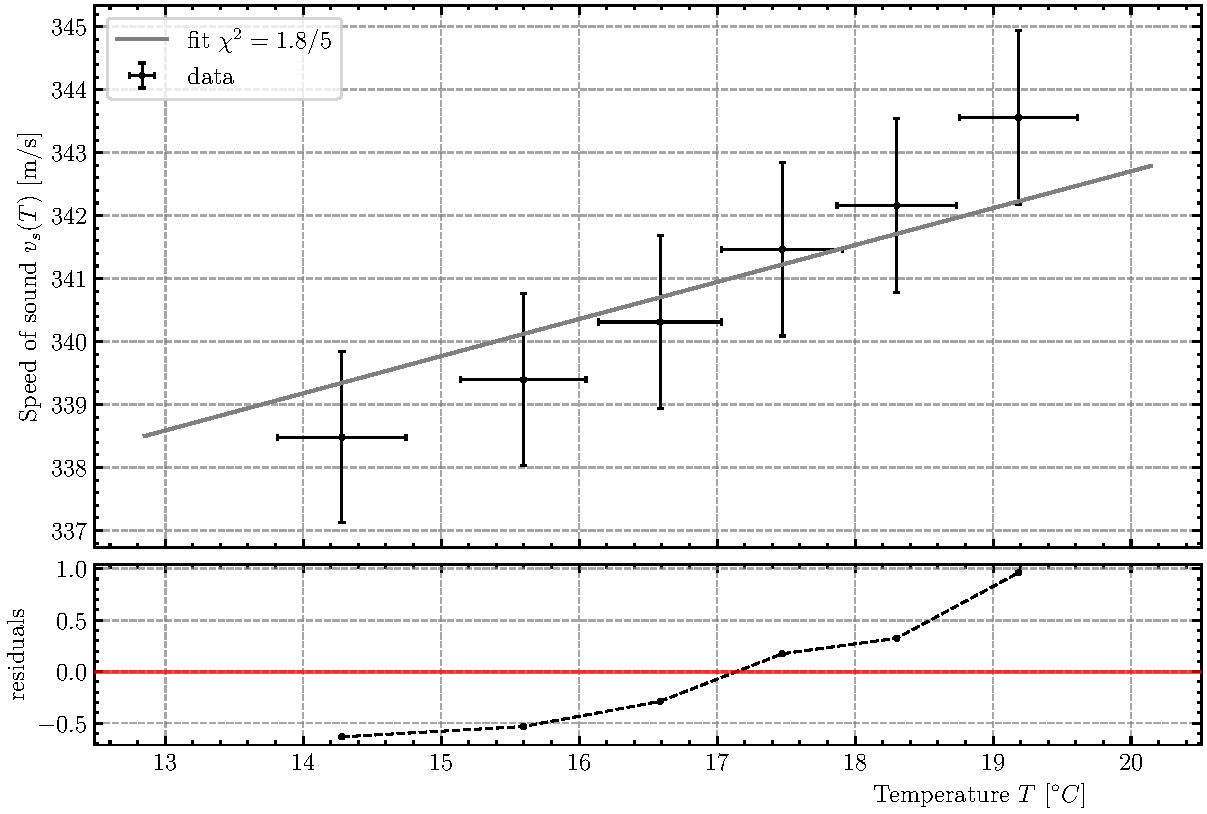
\includegraphics[width=\textwidth]{temptime}
    \caption{Grafico del fit e residui normalizzati per l'andamento della
    velocità del suono in funzione della temperatura}
\end{figure}

Dai risultati del fit abbiamo ottenuto $v_0 = 331 \pm 1 \; \si{\m/\s}$
$(\chi^2/\text{d.o.f} = 1.8/5)$ che risulta pienamente compatibile con il
valore atteso per la velocità del suono in aria $331.45 \; \si{\m/\s}$ a
temperatura $T_0 = \SI{0}{\degreeCelsius}$. 

%=======================
\section*{Conclusioni e commenti finali}
Si è riusciti a dare una misura ragionevole della velocità del suono in aria
e si è riusciti ad apprezzare la sua dipendenza dalla temperatura ambientale
con un semplice sensore ad ultrasuoni ed un termistore.

Nonostante gli esperimenti siano stati svolti in luoghi e condizioni di
temperatura, umidità e altitudine differenti; i risultati trovati risultano
compatibili tra loro e con i valori attesi dalla teoria.

%=======================
\section*{Dichiarazione}
I firmatari di questa relazione dichiarano che il contenuto della relazione \`e
originale, con misure effettuate dai membri del gruppo, e che tutti i firmatari
hanno contribuito alla elaborazione della relazione stessa.

\end{document}
